\documentclass{beamer}

\input{ceesd-macros.tex}

\newif\ifmovies
\moviestrue
%\moviesfalse

\newif\ifsubs
\substrue
%\subsfalse

\newif\ifnotes
\notestrue
%\notesfalse



\begin{document}
  
%======================================================================
\begin{frame}\frametitle{}

\vspace*{0.2in}

\centerline{\textrm{{\huge\bfseries\color{myOrange} Model Document}}} 
\smallskip
\centerline{\textrm{{\large\bfseries\color{myOrange} \textit{Experimental Driver: y0\_euler.py}}}} 
%\centerline{\textrm{{\big\bfseries\color{myOrange} Anatomy of a large scale prediction}}}

\vspace*{0.2in}
\hrule
\begin{center}
\includegraphics[width=0.85\textwidth]{Figures/TitleFig.pdf}
\end{center}
\hrule

\vspace*{0.1in}
\hfill\cPI{Mike Anderson}

\end{frame}
%======================================================================







%======================================================================
\begin{frame}\frametitle{Overview}

\begin{itemize}

\item ACT-II facility, experimental basis
\item Numerical Model
\item Simulation Initialization
\item Sample results

\end{itemize}

\end{frame}

%======================================================================
  
  \begin{frame}\frametitle{ACT-II Experimental Facility}
  
  \vspace*{0.15in}
  \begin{itemize}
  \setlength{\itemsep}{0.15in}
  \item \cPI{ACT-II}:  on-campus AFOSR-funded supersonic combustion facility
  \item Arcjet driven: low cost ($\lesssim$ \$10), low turnaround
    time ($\lesssim$ 10\,min)
   \item direct-connect or free-jet configurations
  \end{itemize}
  \begin{center}
  %\onslide*<1>{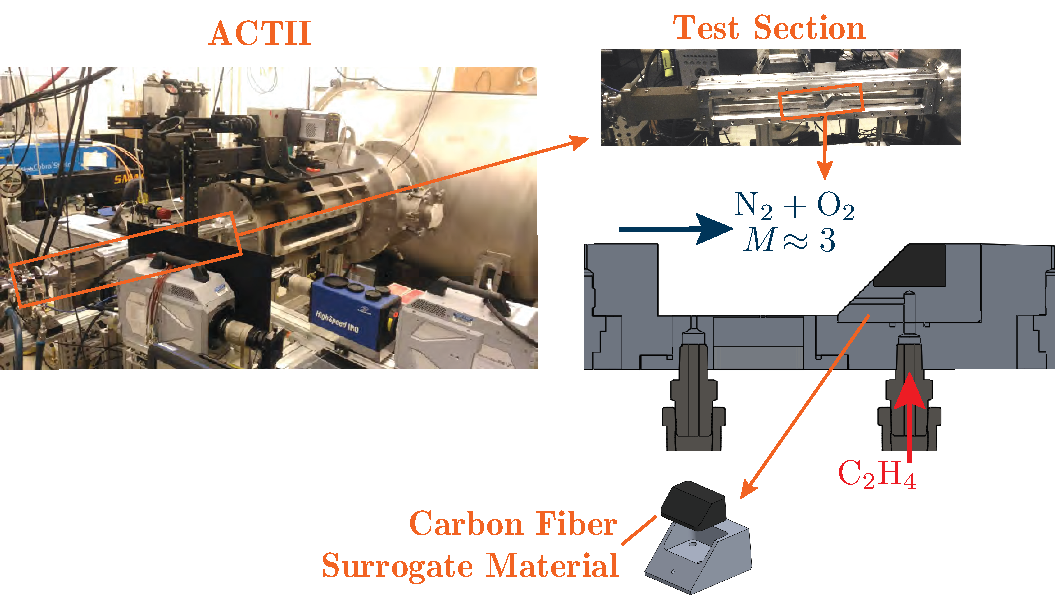
\includegraphics[width=0.9\textwidth]{Figures/actii-y0-setup.pdf}}
  %\onslide*<2>{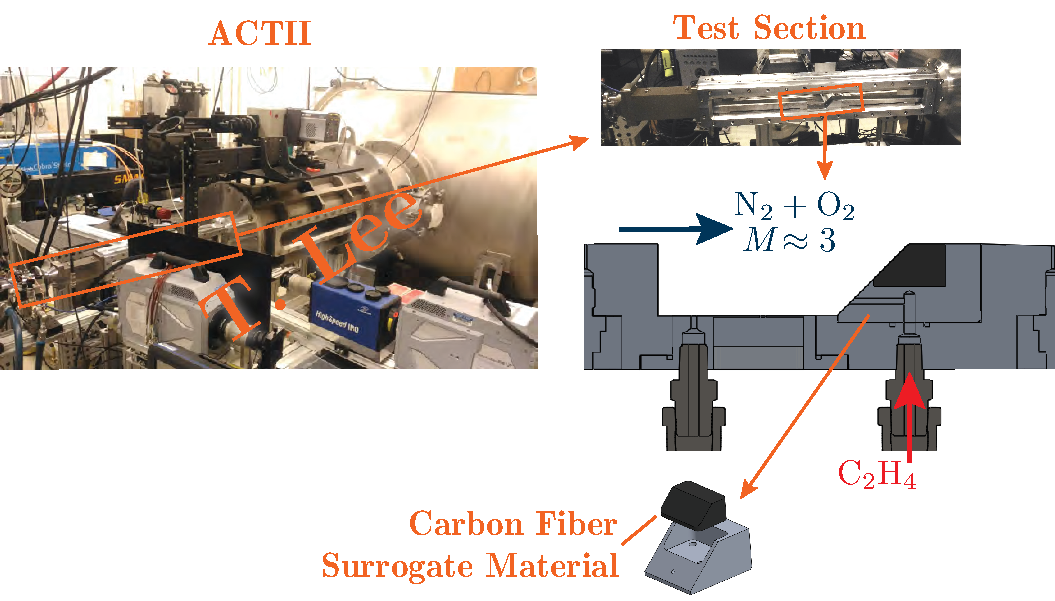
\includegraphics[width=0.9\textwidth]{Figures/actii-y0-setup-NAMES.pdf}}
  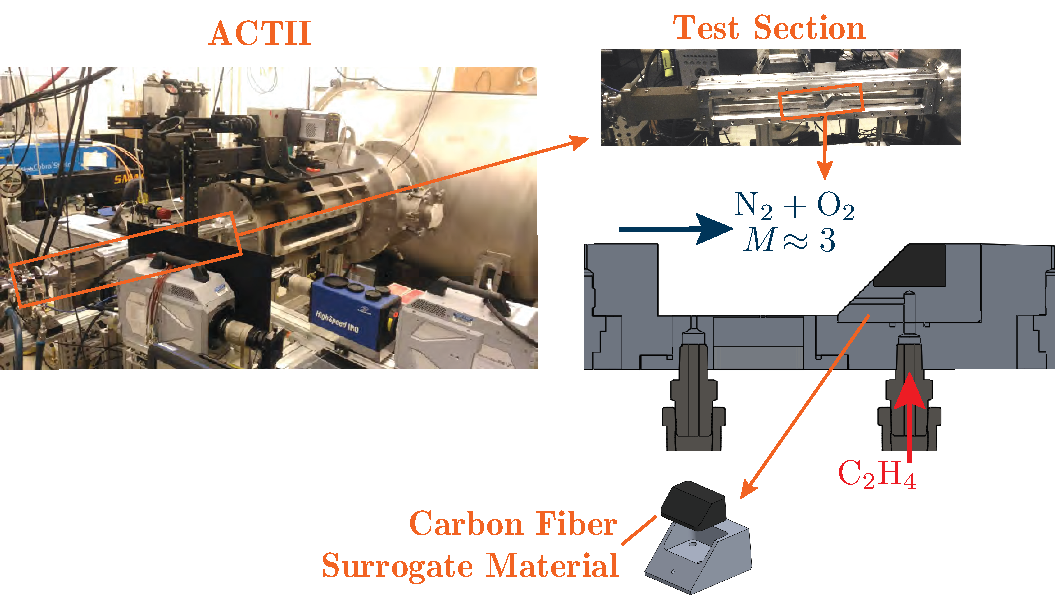
\includegraphics[width=0.9\textwidth]{Figures/actii-y0-setup.pdf}
  \end{center}
  
  \end{frame}
  
  %======================================================================
 
\begin{frame}\frametitle{Experimental Setup - Unstart in a Free-Jet Scramjet}

   \vspace{10pt}
	\begin{minipage}{0.59\textwidth}
	  \begin{itemize}
	    \item ACTII Experimental facility
	    \item Mach 4.5 nozzle
	    \item Varying inlet contraction ratio
	    \item Low ($CO_2$) and high ($O_2/N_2/C_2H_4$) enthalpy runs
	    \item Mass injection or combustion induced unstart
	  \end{itemize}

	  \vspace{-10pt}
	  	\begin{figure}
	  	\centering
	  	%\includegraphics[height=1.75in]{Figures/ACTII.pdf}
	  		\includegraphics[height=1.6in]{Figures/ACTII_testChamber.pdf}
	  	\end{figure}

	\end{minipage}
	\begin{minipage}{0.39\textwidth}
	\begin{figure}
		%\vspace{12pt}
		\centering
	  \includegraphics[height=1.4in]{Figures/scramjetModel.pdf}
	\end{figure}
	
		\begin{singlespace} 
		\tiny Baccarella, Experimental Study of Flow Choking and Inlet Unstart in an Axisymmetric Model Scramjet. 2018. University of Illinois.
		\end{singlespace}
	\end{minipage}


\end{frame}

\begin{frame}\frametitle{Modeling Timeline Y0/Y1}
\cPI {Goal:} \PCtwo~simulations provide Y1 prediction and development milestones for \ceesdcode

\hfill

\cPI{Y0 Target:} October 2020
\begin{itemize}
	\item Low enthalpy, unstart by mass injection
	\begin{itemize}
	\item $CO_2$ flow, $N_2$ injection
	\item 4 port, supersonic injection
	\end{itemize}
\end{itemize}

\cPI{Y1 Target:} Winter 2020/Spring 2021
\begin{itemize}
\item High enthalpy, unstart by mass injection
\begin{itemize}
\item 16 port injector, air injection
\end{itemize}
\item High enthalpy, unstart by combustion
\begin{itemize}
\item 16 port injector, $C_2H_4$ injection, auto-ignition
\end{itemize}
\end{itemize}


\end{frame}
%======================================================================

\begin{frame}\frametitle{Y1 Prediction Targets}

\begin{minipage}{0.49\textwidth}
\cPI{Qualitative}
\begin{itemize}
\item Unstart Go/No-Go
\item PLRS comparison
\end{itemize}

\cPI{Quantitative}
\begin{itemize}
\item Scramjet model pressure
\item Shock/pressure oscillation frequency
\end{itemize}
\end{minipage}
\begin{minipage}{0.49\textwidth}
\centering
\includegraphics[height=1.7in]{Figures/Go-NoGo.pdf}
\end{minipage}

\centering
\includegraphics[width=.7\textwidth]{Figures/PLRS-1.pdf}

\end{frame}



%======================================================================


\begin{frame}\frametitle{Numerical Setup - PlasCom2}

\vspace{10pt}
	\begin{minipage}{0.59\textwidth}
	  \begin{itemize}
	    \item Mesh generation tool based on CAD
	    \item Nine overset meshes
	    \item Variable resolution in nozzle, scramjet model
 	    \begin{itemize}
			\item HalfX - $9.8 M$
			\item OneX - $69 M$
			\item OneX+ - $170 M$
			\item OneX++ - $973 M$
 	    \end{itemize}
	    \item OneX resolution sufficient to resolve inlet shocks and nozzle boundary layer
	    \item Increase scramjet interior resolution to capture turbulence leading to unstart
	  \end{itemize}
	\end{minipage}
	\begin{minipage}{0.39\textwidth}
	\begin{figure}

		\centering
	  \includegraphics[width=2in]{Figures/CAD.pdf}
	\end{figure}
	\vspace{-15pt}
	\begin{figure}
		\centering
 		\includegraphics[width=1.4in]{Figures/inletMesh.pdf}
	\end{figure}
	\end{minipage}
	\begin{figure}
	\centering
	\includegraphics[height=.9in]{Figures/meshPieces.pdf}
	\end{figure}

\end{frame}

\begin{frame}
physics (eqns)
eos (model closure)
boundary conditions (numerical closure)
initialization
sample results
\end{frame}

%\begin{frame}\frametitle{HalfX vs OneX}
%
%  \cPI{Y0 flowthrough}
%  \begin{itemize}
%    \item Qualitative comparison, $2.22x10^{-3} s$
%    \item Constant gamma EOS
%	\end{itemize}
%
%  \begin{figure}
%  \centering
%    \includegraphics[height=2.in]{figures/halfx_v_onex_M.pdf}
%  \end{figure}
%\end{frame}



\begin{frame}\frametitle{Sample Scramjet Interior Pressure?}

   \vspace{10pt}
	\begin{figure}
		%\vspace{12pt}
		\centering
	  \includegraphics[height=1.4in]{Figures/scramjetPressure.pdf}
	\end{figure}

	 \begin{itemize}
	  \item Favorable comparison for initial shock structures
	  \item Under-resolved BL structures?
	 \end{itemize}
	 
\end{frame}
	 

       
	 






%======================================================================
\begin{frame}\frametitle{}

\vspace*{0.2in}

\begin{center}

\includegraphics[width=0.5\textwidth]{Figures/ceesd-logo-2.pdf}

\vspace*{0.35in}
\cPI{\huge Questions?}

\vspace*{0.5in}
\begin{minipage}{0.8\textwidth}
This material is based in part upon work supported by the Department of Energy, National Nuclear Security Administration, under Award Number \textit{TBD}. 
\end{minipage}

\end{center}


\end{frame}
%======================================================================

 

\end{document}


